\section{Methods}\label{section:methods}

\subsection{Neural networks} % (fold)
\label{sub:neural_networks}
\todoyellow{Could easily explain more about everything, but it's kinda out of scope?}
Neural networks is a versatile machine learning model, where data signals are passed through several layers of neurons before a final prediction is made.
An example of such a model can be seen in Figure~\ref{fig:nn}.
The intuition behind this model is, that as the signal is transfered from layer to layer a new representation is created.
The initial layer creates a basic representation, like edges in an image.
The representation are then becoming more and more abstract untill the last layer make a prediction.

A single neuron takes as input the output from the previous layer and a bias value.
These values are multiplied by a trainable weight for each input before being passed to an activation function.

\begin{figure}[H]
    \centering
    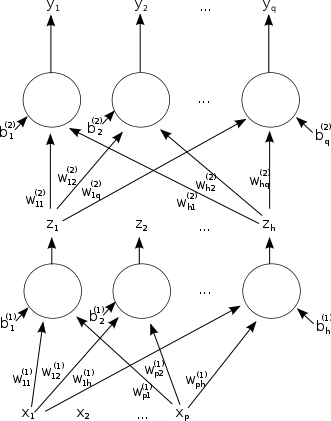
\includegraphics[width=3in]{img/nn.png}
    \caption{Example neural network with two layers}
    \label{fig:nn}
\end{figure}

With neural networks it is often easier to regularize a network instead of tuning the network architecture.


\subsubsection{Convolution} % (fold)
\label{ssub:convolution}
When working with structured data such as images, translation invariance is a very desirable property to have.
To incoorperate this into neural networks, convolutional neural networks were introduced.
Instead of a layer consisting of all the values from the previous layers being passed trough a single neuron, patches of data is passed through different neurons that are sharing the same weights.
This way the network becomes more resistant to moving structures around the data without having to actually include data with structures moved around.

Convolutional neural networks often include pooling layers on the output of the convolution layers.
The pooling layers outputs a statistical summary of the input of a input patch, similar to the concolution patch, defined for the pooling layer.
This is partly used to reduce the output size, but also to select convolution patches with high signal values. \todoyellow{explain maxpooling better}

% subsubsection convolution (end)

\subsubsection{Mini batching} % (fold)
\label{ssub:mini_batching}
To avoid overfitting the training data, it is desireable to not get the true gradiant over all the data.
One method to avoid this, is to use the training data in very small batches, and update the weights using this as an aproximation of the true gradient.

This has the additional benefit, that it speeds up computation dramaticly, as we can get many weight updates from a single pass through the training data.
% subsubsection mini_batching (end)

\subsubsection{Dropout} % (fold)
\label{ssub:dropout}
A regularization technique to avoid overfitting is called dropout.
It works as a layer in between the neural network layers.
The intuition is that with a given probability a input value is set to zero, or otherwise just passed on as it is.
This method helps the network not depend too much on any value from the previous layer, which helps the network be more robust to small changes in the input, as it cannot expect every value to exist.
% subsubsection dropout (end)

\subsubsection{RELU} % (fold)
\label{ssub:relu}
\todoyellow{Droppet leaky relu så det bliver simplere. Skal lige genskrives}
A activation function is almost always part of the setup of a layer.
This function works as a method to introduce nonlinearities to the network.
RELU is a simple activation that is defined as: 
$$RELU(x) = \begin{cases}
    x,              & \text{if } x\geq 0\\
    0,              & \text{otherwise}
\end{cases}$$

One of the problems with this method is, that the gradiant is 0 when below 0.
This can lead to inactive neurons if the output is always negative, if they are initialized badly.
To combat this, the leaky relu function can be used.
It is defined as $$
leakyRELU(x, \alpha) = \begin{cases}
    x,              & \text{if } x\geq 0\\
    \alpha*x,       & \text{otherwise}
\end{cases}$$ 
where alpha is a hyper parameter.
If x is less than 0, it will still learn a little, and can thus escape being always negative.

A positive thing about this function is that the gradiant is also very easy to compute, even though the function is not continues.
It has a gradiant of 1 if above 0 or 0 below.
For leaky relu its gradient is $\alpha$ below 0.
% subsubsection relu (end)

\subsubsection{Softmax} % (fold)
\label{ssub:softmax}
Softmax is another activation function with a very desireable property.
It normalizes the sum of all output to 1.
Before the normalization, the data is used in an exponential function, which helps select high input more than low input.
This makes it a great activation function for the last layer of the network, when working with classification.
% subsubsection softmax (end)

\subsubsection{Autoencoder} % (fold)
\label{ssub:autoencoder}
Autoencoders are an unsupervised neural network structure.
The goal of an autoencoder is to reconstruct it self.
The reconstruction is done after having been pushed through a small layer, so only the most important features are preserved.
The intuition is, that the network consists of a encoder and a decoder.
The encoder tries to encode the data to a selected size, and the decoder then tries to reconstruct the original data from the encoding.

This can be used to generate new data, but this can also be used as a dimensionality reduction technique.
To use it for dimensionality reduction, the encoding is simply the desired output.
The encoder is then simply used as the first layers of the prediction model.

% subsubsection autoencoder (end)

\subsubsection{Mean squared error} % (fold)
\label{ssub:mean_squared_error}
Mean squared error is a loss function.
It simply squares the error, before computing the mean error of all predictions.
This has the benefit that small errors are almost not punished, while big errors are punished more severly.
% subsubsection mean_squared_error (end)

\subsubsection{Categorical cross entropy} % (fold)
\label{ssub:categorical_cross_entropy}
Categorical cross entropy is a loss function for classification.
It optimizes the probability that the correct answer is selected.
This is great because this is indirectly the same as optimizing the accuracy, but with a continues function.
An additional benefit is, that it also improves on uncertain predictions even thouhg they are correct.
A prediction of $51\%$ on the correct category can still be improved alot.

% subsubsection categorical_cross_entropy (end)

\subsubsection{ADAM optimizer} % (fold)
\label{ssub:adam_optimizer}
One of the most widely used optimizer for neural network is some kind of gradient descent.
The idea is to follow the negative gradient untill it flattens out.
With big neural networks, the gradient tends to fluctuate alot while going in a general direction that we want.
To counter this fluctuations and stabalize the optimizer, momentum was introduced to keep the general direction while minimizing small fluctuations.
Adaptive Moment Estimation (Adam) incoorperate momentum together with an adaptive learning rate which has made this a widely used optimizer.
% subsubsection adam_optimizer (end)

\subsubsection{Early stopping} % (fold)
\label{ssub:early_stopping}
To combat overfitting on training data, it can be beneficial to have an external validation training set that is used to validate that the model have not started to overfit.
With early stopping a validation set is scored after each epoch, to validate that the the validation score has not gotten worse.
If the model does not improve validation score after a few epochs, the training is stopped to avoid further overfitting.
% subsubsection early_stopping (end)

\subsubsection{Learning rate decay} % (fold)
\label{ssub:learning_rate_decay}
Having a to high learning rate, it can be hard for the optimizer to find optimal solution, but having a two low learning rate, it will take a long time for it actually reach a solution.
Using learning rate decay, the learning rate will gradually be decreased.
This way the learning rate may be to high initially, but it as the learning rate decreases, it will eventually start to really learn.
% subsubsection learning_rate_decay (end)

% subsection neural_networks (end)

\subsection{Preprocessing} % (fold)
\label{sub:preprocessing}
Often it is a good idea to help prediction by preprocessing the data, to incoorperate domain knowledge into the system, so the model do not have to learn what you already know, or to prepare the data using features not present in the data.
\subsubsection{Normalization} % (fold)
\label{ssub:normalization}
Often it can be hard to compare data from different places in the data space.
To counter this, the data can be normalized with a mean at 0 with standard deviation 1, so data looks the same.
% subsubsection normalization (end)

\subsubsection{Median time filtering} % (fold)
\label{ssub:median_time_filtering}
When using time series it can help to reduce noise, using the time axis.
There are several ways to do it, and simply taking the median of the data of the time axis can help remove fast moving noise, while still keeping the image sharp.

The idea is that fast moving objects and random noise in the data will decline, while slow moving objects will remain in the image.
This will happen in a way such that the noisy outliers will be removed, but the image should still be sharp.
% subsubsection median_time_filtering (end)

% subsection preprocessing (end)
